

As per the given problem, classification needs to be done for k-Nearest Neighbors albeit for the variation of k=2 and k=3 for the two given distance norms (L2 Euclidean and L1 Manhattan) . The Manhattan distance is given by L1 absolute value and the Euclidean distance is given by the L2 norm.
 The respective first three nearest distances are colored for the given specific points and then the further classification is done for the nearest neighbor. For k=2, the two least distances are chosen while for the k=3, the least 3 are chosen for classification. Ties are broken randomly.Given points are:
\begin {enumerate}
	\item( 4,3,3)   
	\item( 4,-1,1)  
	\item(-2,4,5)   
	\item(-2,-6,-1) 
	\item( 6,0,2)  
\end {enumerate}
The two distances are tabulated in two separate tables as below and the minimum is found out respectively.
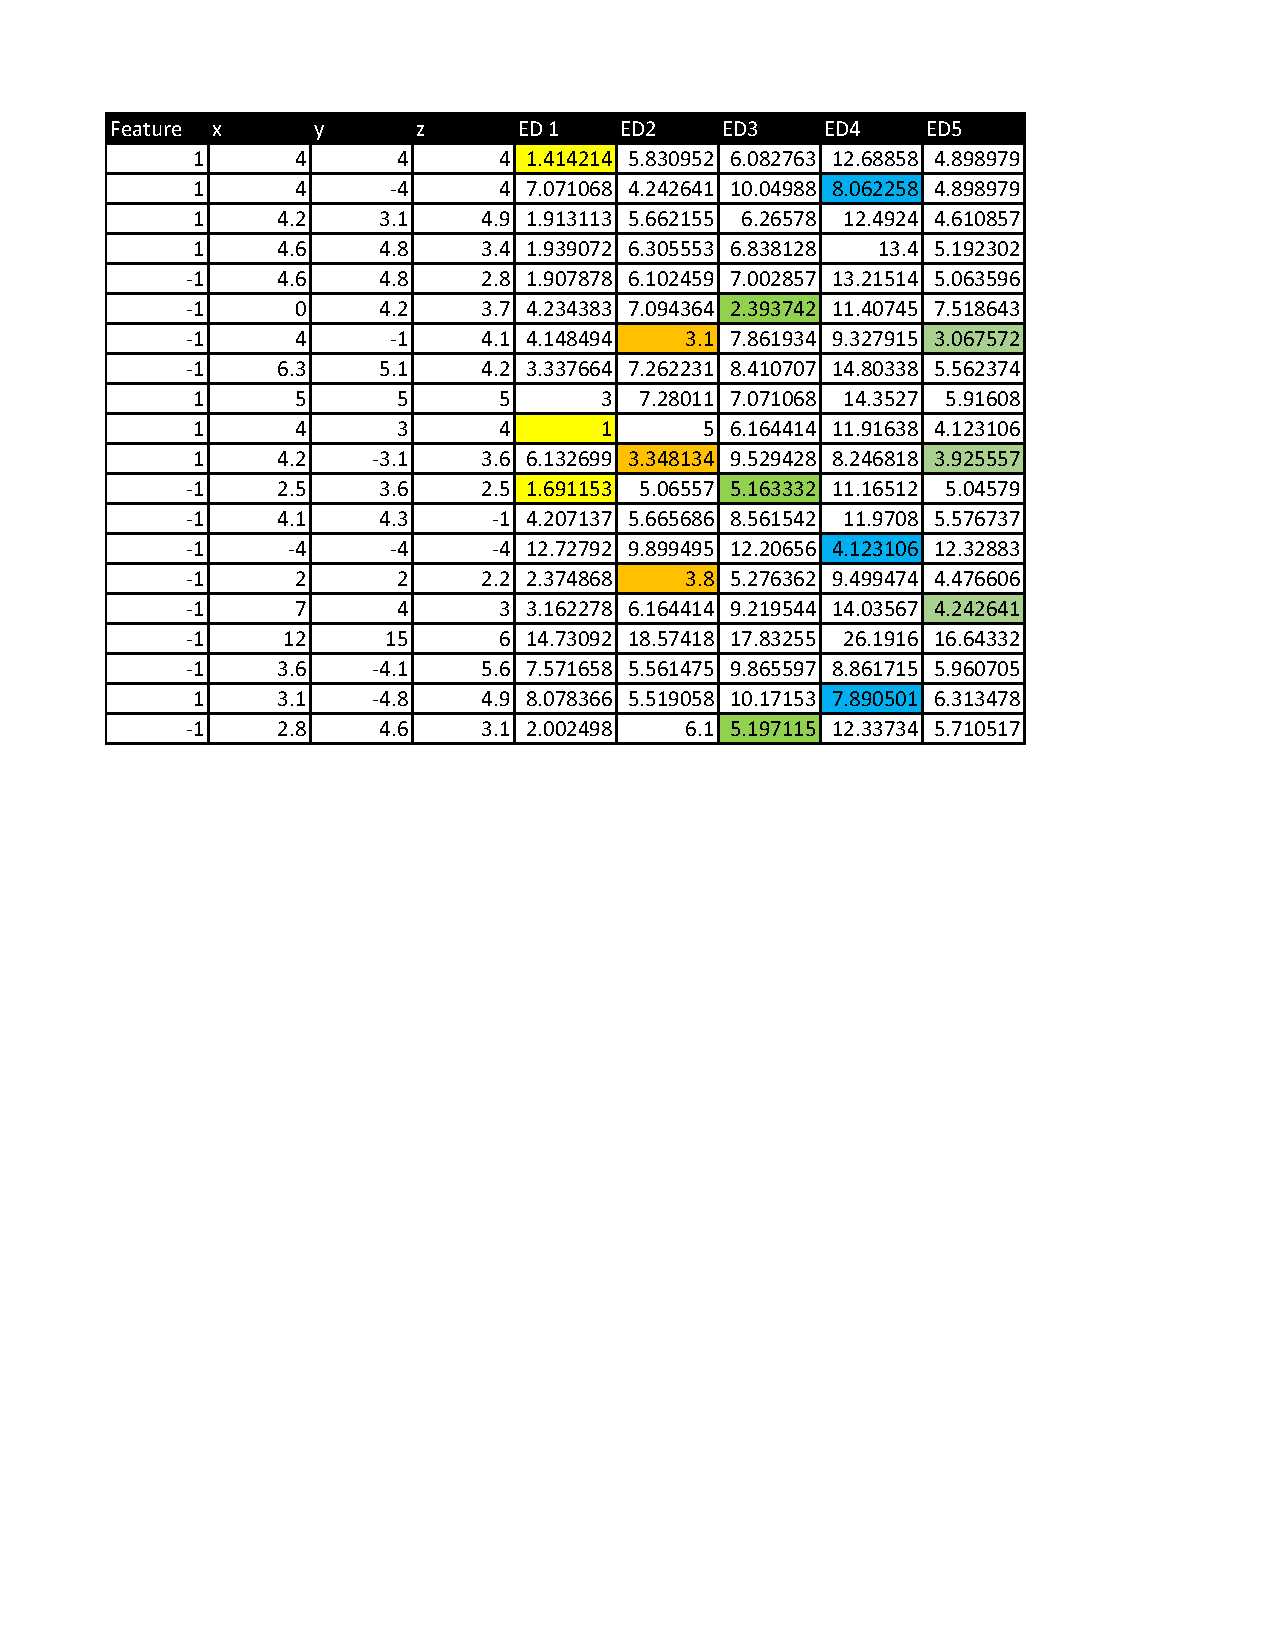
\includepdf[scale=0.8]{ALds1.pdf}
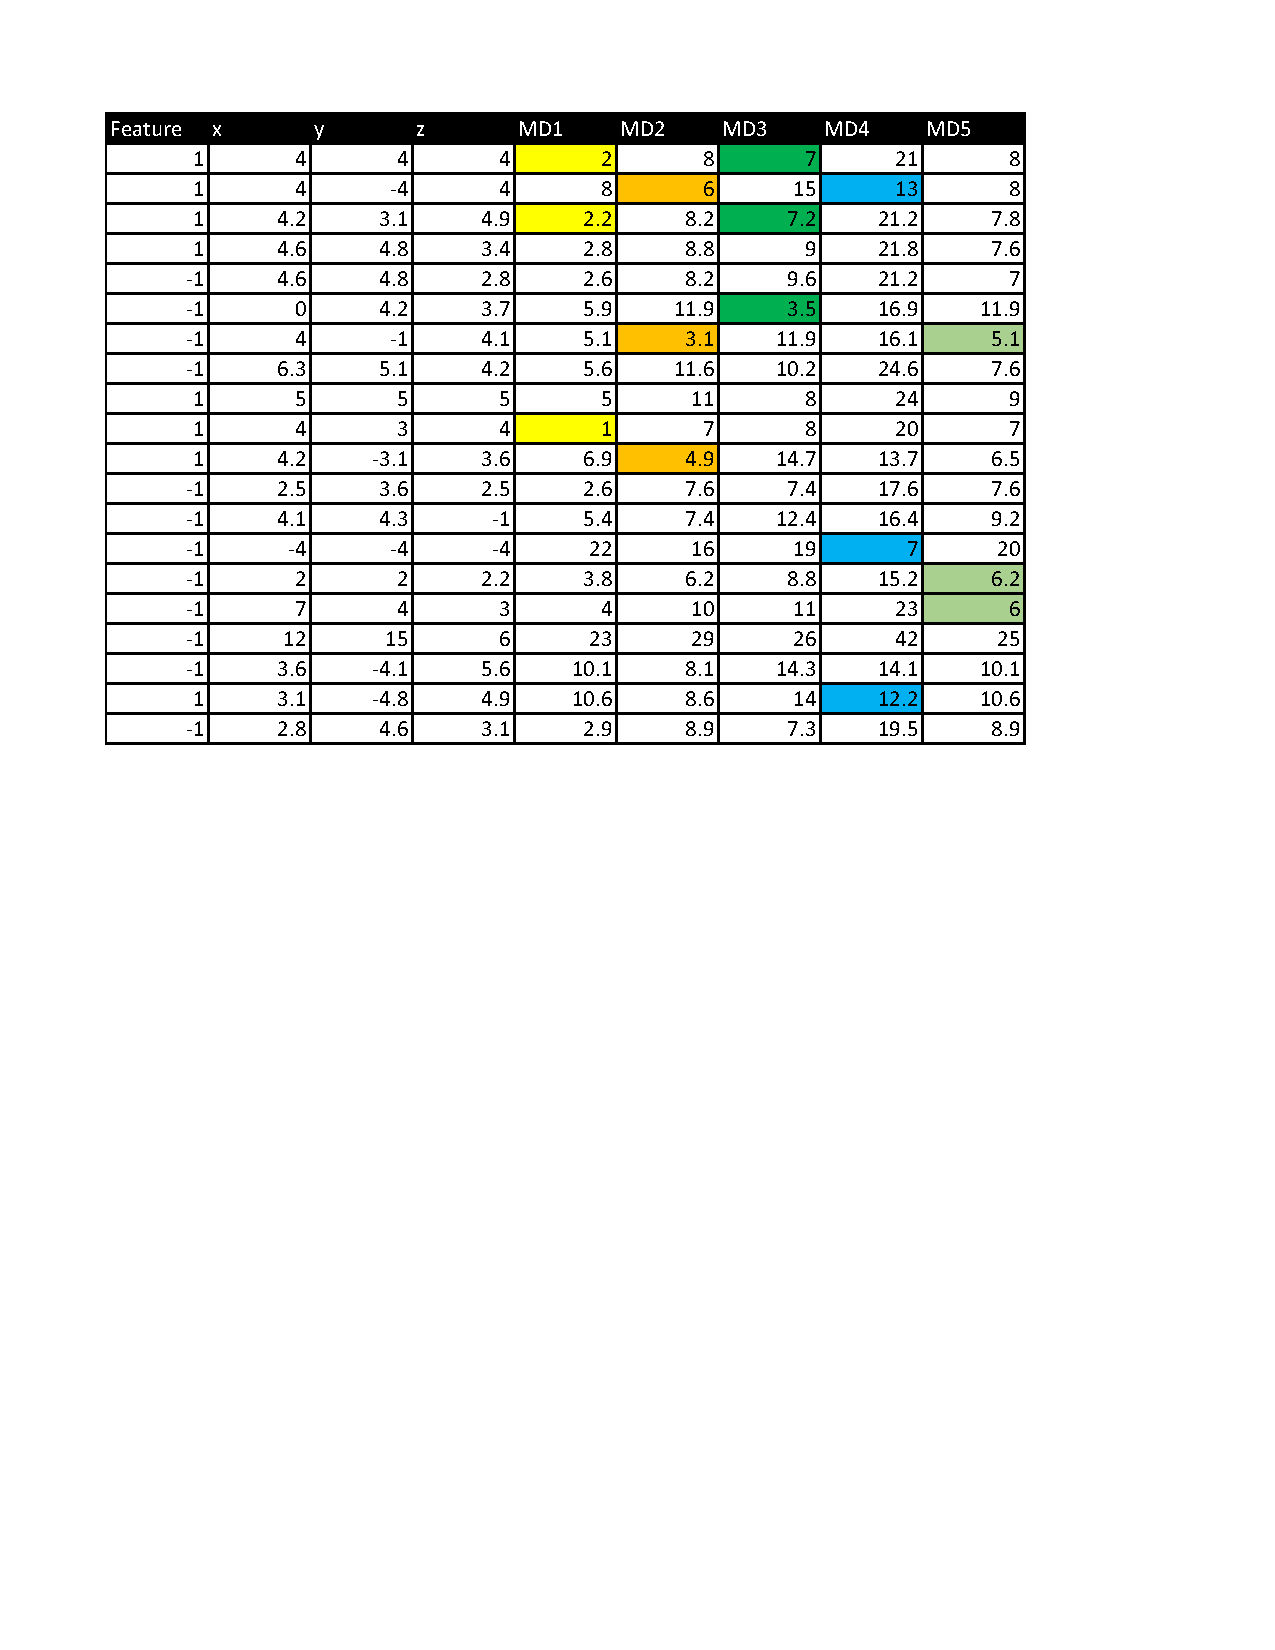
\includepdf[scale=0.8]{ALds2.pdf}
For k=2 and k= 3 respectively, the feature classification for the given points with respect to Manhattan distance is respectively:
\begin {enumerate}
	\item( 4,3,3)      1 /1
	\item( 4,-1,1)    -1/ 1
	\item(-2,4,5)     -1/ 1
	\item(-2,-6,-1)    1/ 1
	\item( 6,0,2)      -1/-1
\end {enumerate}
For k=2 and k= 3 respectively, the feature classification for the given points with respect to Euclidean distance is respectively:
\begin {enumerate}
	\item( 4,3,3)     1 /  1
	\item( 4,-1,1)   -1/ -1
	\item(-2,4,5)    -1/ -1
	\item(-2,-6,-1)   1 / 1
	\item( 6,0,2)      1/ -1
\end {enumerate}
